%- - - - - - - - - - - - - - - - - - - - - - - - - - - - - - - - - SLIDE -
\begin{frame}
\frametitle{Como Se Preparar?}
\begin{block}{}
Para estar bem preparado para participar dessas competições é necessário passar por varias etapas:
\begin{enumerate}
	\item Escolher uma linguagem;
	\begin{itemize}
		\item Dominar sintaxe, comandos básicos e as funções mais usadas em competições.
	\end{itemize}
	\item Aprender noções de Complexidade de Algoritmos;
	\begin{itemize}
		\item Calcular complexidade de tempo e memória e estimar o tempo de execução;
	\end{itemize}
	\item Dominar as estruturas de dados básicas;
	\begin{itemize}
		\item Vetores, strings, pilha, fila, etc.
	\end{itemize}
	\item Dominar Entrada e Saída;
	\begin{itemize}
		\item Leitura dos diferentes tipos, formatação de sáida.
	\end{itemize}
	\item Dominar algoritmos clássicos e técnicas comuns para resolução de problemas .
\end{enumerate}
\end{block}
\end{frame}

%- - - - - - - - - - - - - - - - - - - - - - - - - - - - - - - - - SLIDE -
\begin{frame}
\frametitle{Como Se Preparar?}
\begin{block}{Alguns exemplos de algoritmos clássicos e técnicas comuns}
\begin{itemize}	
	\item Recursão, Backtracking
	\begin{itemize}
		\item	Saber enumerar permutações, combinações e arranjos.
	\end{itemize}
	\item Grafos
	\begin{itemize}
		\item Estruturas de dados para representá-los; Algoritmos de busca: BFS, DFS; Árvore Geradora Mínima; Caminhos mínimos.
	\end{itemize}
	\item Programação Dinâmica
	\begin{itemize}	
		\item Entender a idéia e conhecer os problemas clássicos.
	\end{itemize}
	\item Matemática
	\begin{itemize}	
		\item Conceitos de combinatória, probabilidade, cálculo e teoria dos números.
	\end{itemize}
	\item Geometria / Geometria Computacional
	\item Algoritmos gulosos, divisão e conquista, estruturas de dados, ...
\end{itemize}
\end{block}
\end{frame}

%- - - - - - - - - - - - - - - - - - - - - - - - - - - - - - - - - SLIDE -
\begin{frame}
\frametitle{Como Se Preparar?}
\begin{block}{E como dominar essas técnicas?}
\begin{itemize}	
	\item Estudando as mesmas em livros, artigos e tutoriais encontrados na internet;
	\item Praticando em Online Judges;
	\begin{itemize}
		\item Existem várias páginas na internet onde é possível resolver problemas no estilo da maratona e conferir se sua solução está correta.
	\end{itemize}
	\item Participando de competições online;
	\begin{itemize}
		\item Vários Online Judges organizam competições para que os competidores possam treinar.
		\item Sites como topCoder, Codeforces e Codechef organizam competições regularmente.
	\end{itemize}
	\item Esclarecendo dúvidas e pedindo ajuda a competidores mais experientes.
\end{itemize}
\end{block}
\end{frame}

%- - - - - - - - - - - - - - - - - - - - - - - - - - - - - - - - - SLIDE -
\begin{frame}
\frametitle{Como Se Preparar?}
\begin{block}{Material para estudo - Livros voltados	 para competições}
\begin{itemize}
		\item Competitive Programming 2: This increases the lower bound of Programming Contests. Again. - Steven Halim, Felix Halim
		\item Programming Challenges - Steven S. Skiena, Miguel A. Revilla 
		\item The Art of Algorithms and Programming Contests. - Rujia Liu, Liang Huang 
		\item Art of Programming Contest - Ahmed Shamsul Arefin
\end{itemize}
\end{block}
\end{frame}

%- - - - - - - - - - - - - - - - - - - - - - - - - - - - - - - - - SLIDE -
\begin{frame}
\frametitle{Como Se Preparar?}
\begin{block}{Material para estudo - Referências para desenvolvimento de algoritmos}
\begin{itemize}
	\item Introduction to Algorithms. Thomas H. Cormen, Charles E. Leiserson, Ronald L. Rivest. MIT Press/MacGraw Hill, 1990. 
	\item Introduction to Algorithms: A Creative Approach. Udi Manber. Addison-Wesley, 1989. 
	\item Algorithms in C Parts 1-5. Robert Sedgewick. 3rd. Edition, vol. 1. Addison Wesley Longman, 1998. 
	\item Computational geometry: An introduction. F.P. Preparata and M.I. Shamos. Texts and Monographs in Computer Science, Springer-Verlag, New York, 1985. 
\end{itemize}
\end{block}
\end{frame}

%- - - - - - - - - - - - - - - - - - - - - - - - - - - - - - - - - SLIDE -
\begin{frame}
\frametitle{Como Se Preparar?}
\begin{block}{Material para estudo - Referências para desenvolvimento de algoritmos}
\begin{itemize}
	\item Grafos e Algoritmos Computacionais. J. L. Szwarcfiter. Campus, Rio de Janeiro, 1986. 
	\item Data Structures and Algorithms. Alfred V. Aho, Jhon E. Hopcroft and Jeffrey Ullman Addison Wesley, 1983. 
	\item Concrete Mathematics. Donald E. Knuth, Ronald L. Graham and O. Patashnik. 2nd Edition Addison-Wesley, 1994. 
	\item Computational Complexity. Papadimitriou, C.H., Addison-Wesley, 1993. 
\end{itemize}
\end{block}
\end{frame}

%- - - - - - - - - - - - - - - - - - - - - - - - - - - - - - - - - SLIDE -
\begin{frame}
\frametitle{Como Se Preparar?}
\begin{block}{Material para estudo - Uma ``bibliografia'' indicada}
\begin{itemize}
	\item Competitive Programming 2 - Steven Halim, Felix Halim
	\begin{center}
	
\includegraphics[width=.2\textwidth]{figuras/cp2.png}\\
	\tiny\url{https://sites.google.com/site/stevenhalim/}
	\end{center}
	
	\item \url{http://www.ime.usp.br/~pf/algoritmos_para_grafos/}
	\item \url{http://www.cplusplus.com/reference/}	
\end{itemize}
\end{block}
\end{frame}


%- - - - - - - - - - - - - - - - - - - - - - - - - - - - - - - - - SLIDE -
\begin{frame}
\frametitle{Como Se Preparar?}
\begin{block}{Online judges - A lista é extensa...}
\begin{itemize}
	\item URI Online Judge - \url{http://www.urionlinejudge.com.br/}
	\item UVa -- \url{http://uva.onlinejudge.org/}
	\item Live Archive -- \url{http://livearchive.onlinejudge.org/}
	\item SPOJ -- \url{http://www.spoj.pl/}
	\item TJU -- \url{http://acm.tju.edu.cn/toj/}
	\item SGU -- \url{http://acm.sgu.ru/}
	\item PKU -- \url{http://poj.org/}
	\item Timus -- \url{http://acm.timus.ru/}
	\item ZOJ -- \url{http://acm.zju.edu.cn/onlinejudge/}
	\item SPOJ BR  -- \url{http://br.spoj.pl/}
	\item USACO -- \url{http://train.usaco.org/usacogate}
	\item $\infty$
\end{itemize}
\end{block}
\end{frame}

%- - - - - - - - - - - - - - - - - - - - - - - - - - - - - - - - - SLIDE -
\begin{frame}
\frametitle{Como Se Preparar?}
\begin{block}{Online judges - Por once começar}
\begin{itemize}
	\item URI Online Judge - \url{http://www.urionlinejudge.com.br/}
	\begin{itemize}
		\item Portal brasileiro bastante didático com problemas em português e inglês classificados de acordo com a dificuldade e a possível técnica envolvida na solução.
	\end{itemize}
	\item SPOJ BR  -- \url{http://br.spoj.pl/}
		\begin{itemize}
		\item Página com problemas em português, de seletivas, regionais e nacionais passadas. Seção com problemas da OBI pode ser bastante interessante para alunos iniciantes.
	\end{itemize}
	\item USACO -- \url{http://train.usaco.org/usacogate}
	\begin{itemize}
		\item Curso de treinamento para os alunos dos Estados Unidos interessados em participar da olimpíada de informática. Dividido em seções, textos breves explicando técnicas e fornecendo mais referências e listas de problemas para serem resolvidos.
	\end{itemize}
\end{itemize}
\end{block}
\end{frame}

%- - - - - - - - - - - - - - - - - - - - - - - - - - - - - - - - - SLIDE -
\begin{frame}
\frametitle{Como Se Preparar?}
\begin{block}{Online judges - Partindo para problemas mais desafiadores}
\begin{itemize}
	\item SPOJ -- \url{http://www.spoj.pl/}	
	\begin{itemize}
		\item Coleção vasta de problemas com enunciados em inglês de origens e dificuldades variadas.
	\end{itemize}
	\item Live Archive -- \url{http://livearchive.onlinejudge.org/}
	\begin{itemize}
		\item Coleção de problemas das provas de regionais e finais mundiais passadas.
	\end{itemize}
	\item UVa -- \url{http://uva.onlinejudge.org/}
\end{itemize}
\end{block}
\end{frame}

%- - - - - - - - - - - - - - - - - - - - - - - - - - - - - - - - - SLIDE -
\begin{frame}
\frametitle{Como Se Preparar?}
\begin{block}{Online judges - Ferramentas}
\begin{itemize}
	\item Virtual Online Contests -- \url{http://ahmed-aly.com/voc/}
	\begin{itemize}
		\item Permite criar placares para competições envolvendo problemas de vários juízes e acompanhar quais problemas os usuários resolveram. Também tem vários outros recursos, como buscar por problemas de acordo com a técnica envolvida na solução e criar times e grupos.
	\end{itemize}
	\item uHunt -- \url{http://uhunt.felix-halim.net/}	
	\begin{itemize}
		\item Ferramenta para o UVa online-judge que gera estatísticas dos problemas resolvidos por cada usuário e dá sugestões de quais problemas resolver. Criado por um dos autores do livro Competitive Programming facilita bastante encontrar e manter um histórico de quais dos problemas discutidos no livro já foram resolvidos.
	\end{itemize}
\end{itemize}
\end{block}
\end{frame}

%- - - - - - - - - - - - - - - - - - - - - - - - - - - - - - - - - SLIDE -
\begin{frame}
\frametitle{Como Se Preparar?}
\begin{block}{Competições Online}
\begin{itemize}
	\item TopCoder SRMs -- \url{http://topcoder.com/tc}
	\item Codeforces -- \url{http://codeforces.com/contests}
	\item Codechef -- \url{http://codechef.com/}
	\item TopCoder Open -- \url{http://community.topcoder.com/tco13/}	
	\item Google Code Jam -- \url{http://code.google.com/codejam/}
	\item Facebook Hacker Cup -- \url{https://www.facebook.com/hackercup}
	\item IPSC -- \url{http://ipsc.ksp.sk/}
	\item \bf{Calendário de competições} -- \url{http://codingdoor.com/}
\end{itemize}
\end{block}
\end{frame}

%- - - - - - - - - - - - - - - - - - - - - - - - - - - - - - - - - SLIDE -
\begin{frame}
\frametitle{Como Se Preparar?}
\begin{block}{Competições Online -- TopCoder}
\begin{itemize}
	\item TopCoder SRMs -- \url{http://topcoder.com/tc}
	\begin{itemize}
		\item Geralmente ocorrem de 15 em 15 dias. 
		\item Competidores recebem uma pontuação e são rankeados e separados em divisões. Div. 2 tem problemas mais simples, a medida que o competidor vai apresentando um bom desempenho sua pontuação aumenta e ele passa a competir na div. 1 onde os problemas são mais desafiadores.
		\item Competição dividida em fases: Coding Phase, Challenge Phase e System Test.
		\item Explicações das soluções para os problemas divulgadas algum tempo após a competição.
	\end{itemize}
\end{itemize}
\end{block}
\end{frame}

%- - - - - - - - - - - - - - - - - - - - - - - - - - - - - - - - - SLIDE -
\begin{frame}
\frametitle{Como Se Preparar?}
\begin{block}{Competições Online -- TopCoder}
\begin{center}
	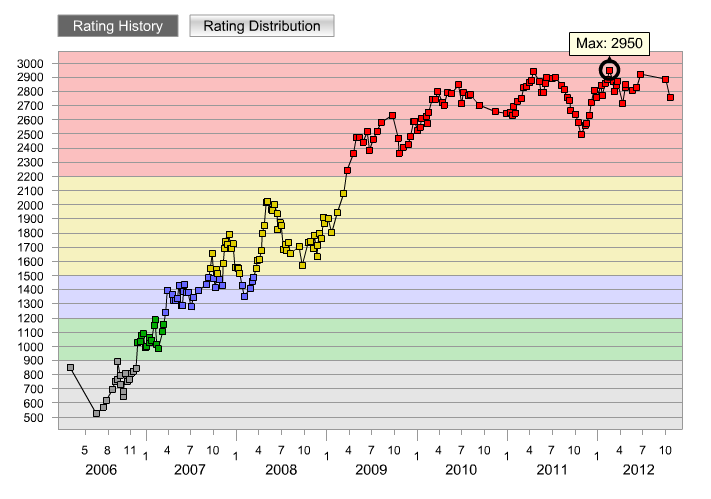
\includegraphics[width=.7\textwidth]{figuras/tcrating.png}
\end{center}
\end{block}
\end{frame}
	
%- - - - - - - - - - - - - - - - - - - - - - - - - - - - - - - - - SLIDE -	
\begin{frame}
\frametitle{Como Se Preparar?}
\begin{block}{Competições Online -- Codeforces}
\begin{itemize}	
	\item Codeforces -- \url{http://codeforces.com/contests}
	\begin{itemize}
		\item Competições semelhantes as do topCoder, porém com mais problemas e maior duração. Os competidores são separados em duas divisões e as competições tem duas etapas, Coding Phase e System Test.
		\item Explicações das soluções para os problemas geralmente são divulgadas algum tempo após a competição.
	\end{itemize}
\end{itemize}
\end{block}
\end{frame}

%- - - - - - - - - - - - - - - - - - - - - - - - - - - - - - - - - SLIDE -
\begin{frame}
\frametitle{Como Se Preparar?}
\begin{block}{Competições Online -- Codechef}
\begin{itemize}	
	\item Codechef -- \url{http://codechef.com/}
	\begin{itemize}
		\item Dois tipos de competições, ambas sem distinção entre os competidores.
		\begin{itemize}
			\item Long Contests -- Competição mais didática e de longa duração, acontece todos os meses a partir do dia primeiro e tem duração de 10 dias. A prova é composta por 10 problemas de dificuldades variadas e o objetivo é que o competidor tenha tempo de pesquisar e aprender novas técnicas para resolver os problemas propostos. 
			\item Short Contests -- Competições curtas, com 2,5 horas de duração que acontecem uma vez por mês. A prova tem 5 questões de dificuldades variadas.
		\end{itemize}
		\item Explicações das soluções sempre são divulgadas pouco tempo depois das competições.
	\end{itemize}
\end{itemize}
\end{block}
\end{frame}

%- - - - - - - - - - - - - - - - - - - - - - - - - - - - - - - - - SLIDE -
\begin{frame}
\frametitle{Como Se Preparar?}
\begin{block}{Entrar em contato com outros competidores}
\begin{itemize}	
	\item Praticamente todos os Online Judges tem fóruns onde os usuários podem trocar informações e dicas sobre os problemas, é importante usar bastante essa ferramenta.
	\item \url{http://br.groups.yahoo.com/group/maratona/} -- Grupo nacional da maratona no Yahoo Grupos, lugar onde competidores de todo o Brasil podem discutir sobre resoluções de problemas e competições de programação.
	\item \url{https://www.facebook.com/groups/maratonago/} -- Grupo destinado a alunos, professores, ex-competidores e entusiastas da Maratona de Programação no estado de Goiás. 
\end{itemize}
\end{block}
\end{frame}

%- - - - - - - - - - - - - - - - - - - - - - - - - - - - - - - - - SLIDE -
%\begin{frame}
%\frametitle{Como Se Preparar?}
%\begin{block}{Mais alguns endereços \dots}
%\begin{itemize}
%	\item \url{https://sites.google.com/site/obiufg/Principal} -- Página do treinamento da OBI oferecido pelo INF-UFG, livro preparatório para OBI pode ser encontrado nesse link.
%	\item \url{http://www.ime.usp.br/~cassio/boca/} -- site do BOCA
%\end{itemize}
%\end{block}
%\end{frame}

%- - - - - - - - - - - - - - - - - - - - - - - - - - - - - - - - - SLIDE -
%\begin{frame}
% \frametitle{\em Universidade de Valladolid}
% \begin{block}{}%{Online Judge}
%  \centering
%  \includegraphics[width=.95\textwidth]{figuras/uva-online-judge}
% \end{block}
%\end{frame}